\chapter{Opstilling}
\label{cha:opstilling}

En stråle af protoner accelereres op til den ønskede energi med en 5\MV Van de Graaf
accelerator. Strålen afbøjes med en eletromagnet og sendes ind i \beamline, hvor den først passerer
gennem et hul i midten af den ene detektor. En del af strålen vil kollidere med et
\SI[per-mode = symbol]{20}{\micro\gram\per\cm\squared} \Bor-\target placeret på
\SI[per-mode = symbol]{4}{\micro\gram\per\cm\squared} kulstof bagbeklædning.  Den resterende del af
strålen vil passere videre gennem \beamline, hvor det igen vil passere gennem en anden detektor for
at ende i et Faradaybæger. Opstillingen er skitseret på \cref{fig:opstilling}.
\begin{figure}[h]
  \centering
  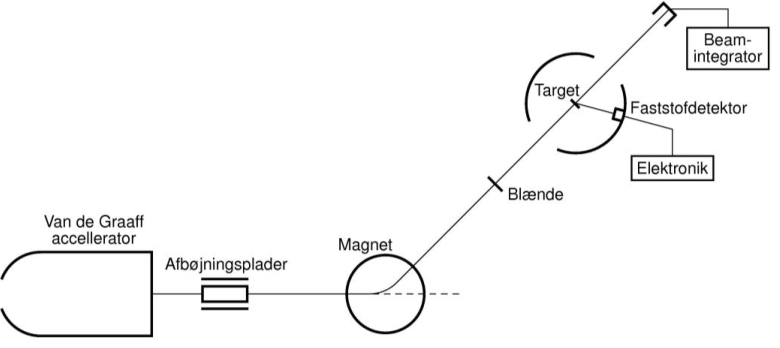
\includegraphics[width=0.7\columnwidth]{Opstilling}
  \caption{Skematisk tegning af opstillingen. Figuren er lånt fra \cite{Knudsen}.}
  \label{fig:opstilling}
\end{figure}

Detektorsystemet består af to cirkulære dobbeltsidede silicium strip detektorer (DSSSD) af typen S3 fra Micron
Semiconductors Limited \cite{micron-s3}.  Disse fungerer på samme måde som almindelige
faststofdetektorer og en skematisk tegning af detektoren ses på \cref{fig:S3}.  Fordelen ved disse
detektorer er opdelingen af forsiden og bagsiden i et antal områder, kaldet strips. Hermed er det
muligt at optage et positionsfølsomt spektrum af partiklerne. Bagsiden er opdelt i 32 radiale
sektorer. Forsiden er opdelt i en række ringe, der hver er 886\um tykke og adskilles af et
100\um isolerende område.
\begin{figure}[hbt]
  \setlength{\textfloatsep}{0pt plus 1.0pt minus 2.0pt}
  \centering
  \subbottom[W1 dektoren med 16 vertikale og horisontale sektorer.]{%
    \raisebox{0cm}{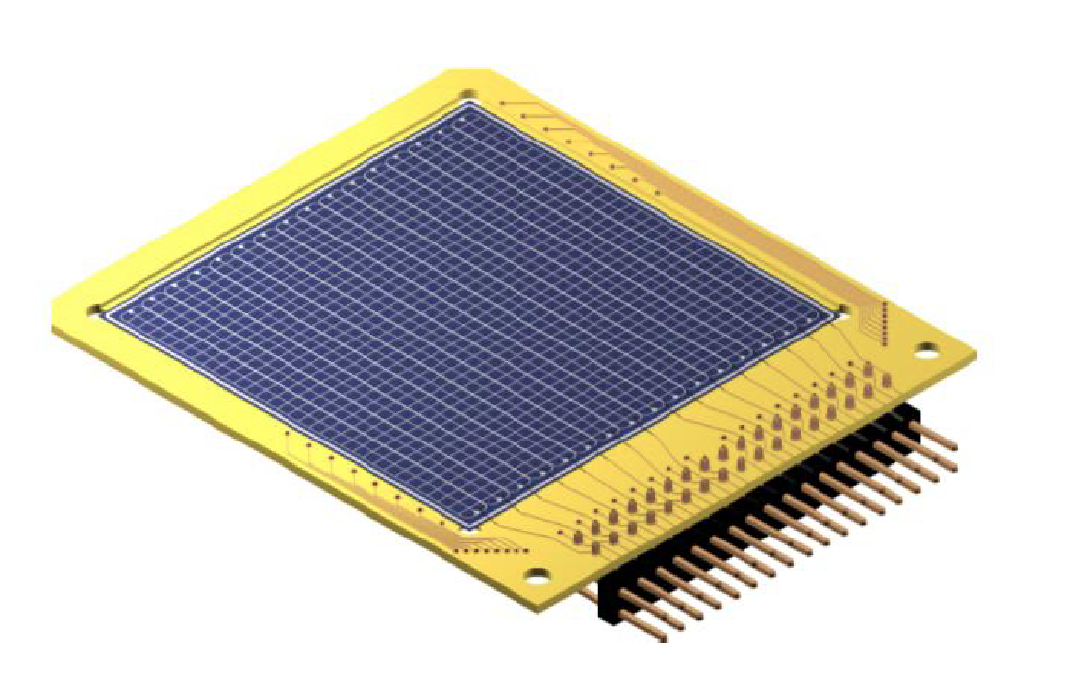
\includegraphics[width=0.44\columnwidth]{W1}}}%
  %
  \hfill
  \subbottom[S3 detektoren med 24 ringe og 32 sektorer.]{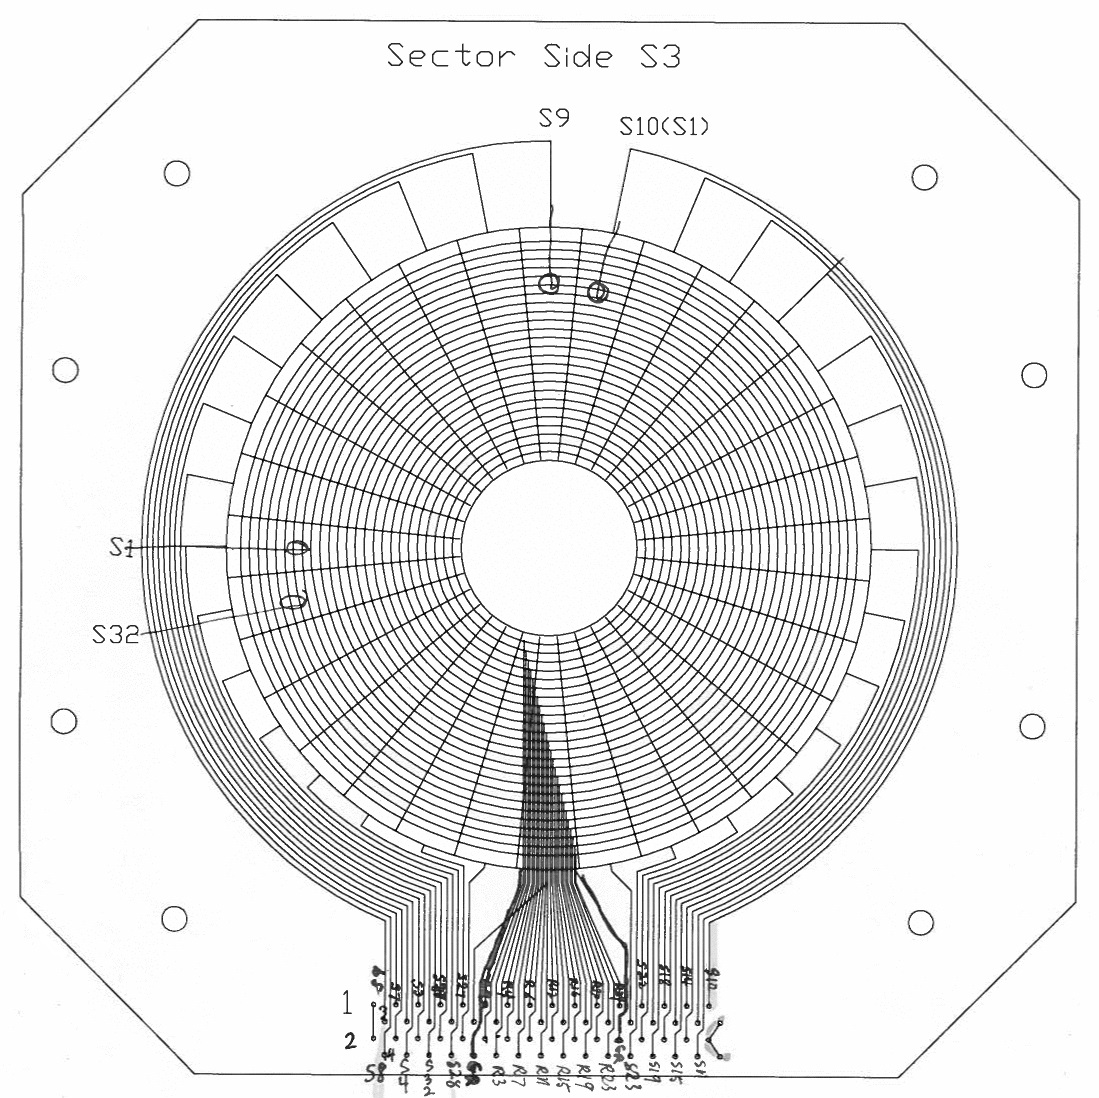
\includegraphics[width=0.35\columnwidth]{S3}}%
  % \fxfatal{Her mangler en tegning af W1-detektoren}
  % 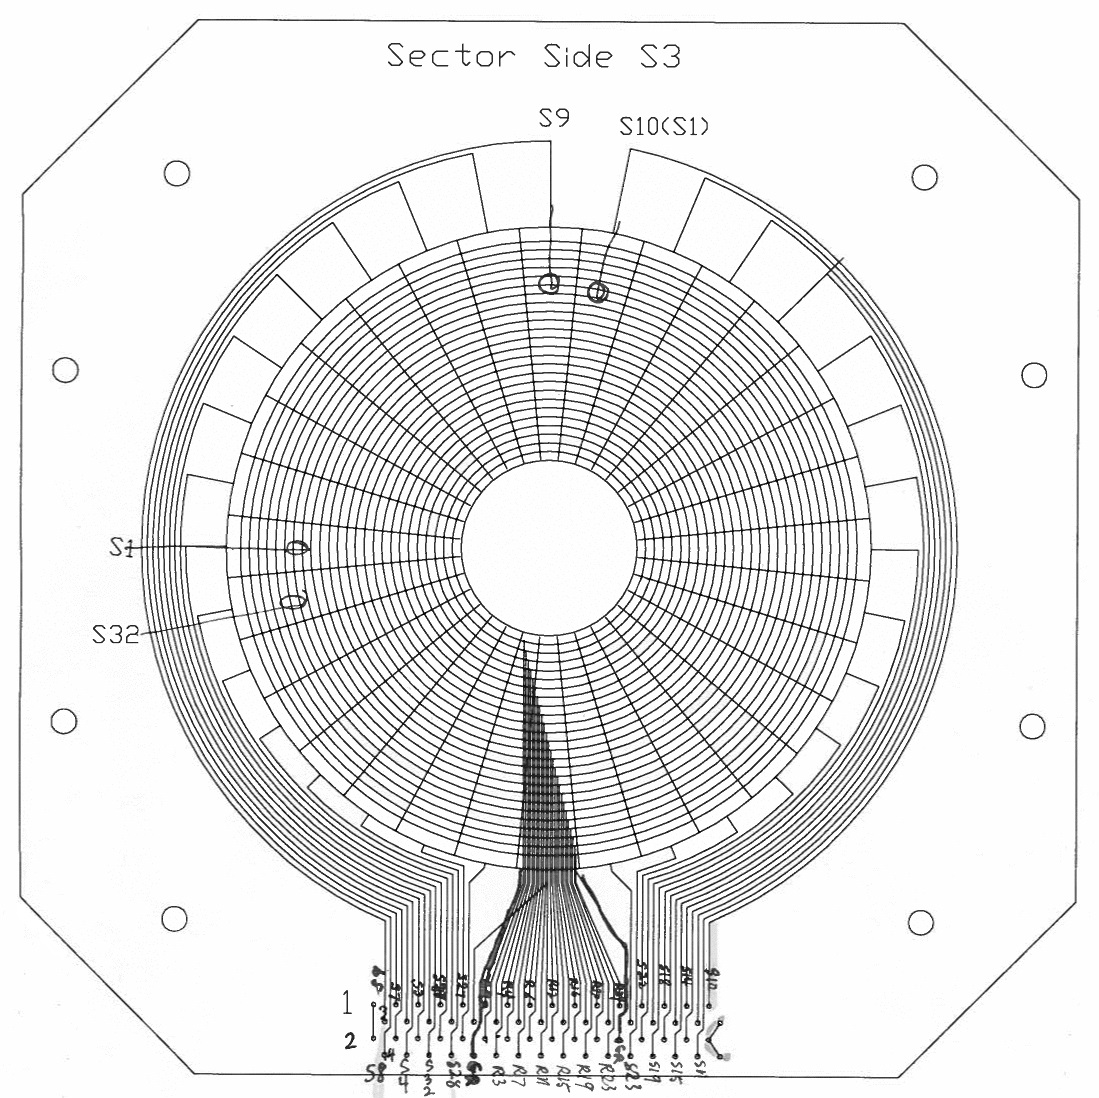
\includegraphics[width=0.5\columnwidth]{S3}
  \caption{Skematisk tegning af de to detektortyper. Bemærk at de forskellige sektortyper er
    placeret på hver sin side af detektoren.}
  \label{fig:S3}
\end{figure}

Den første detektor, som strålen passerer igennem, vil blive omtalt som detektor 4 og den udspænder
polarvinklerne, målt ifht. \beamline, fra $141\degree$ til $165\degree$. Den anden detektor benævnes
med detektor 3 og den udspænder fra $15\degree$ til $40\degree$. Placeringen af de enkelte
detektorer er skitseret på \cref{fig:detektordistro}a.

På begge sidder er der endvidere placeret to W1 DSSSD detektorer, også fra Micron
\cite{micron-W1}. Disse dektorer er firkantede og det aktive område måler
${\SI{49.5}{\mm} \times \SI{49.5}{\mm}}$. De to sider er opdelt i 16 strips af \SI{3}{\mm} 
adskilt af et \SI{0.1}{\mm} isolerende område. Strips'ne på forsiden og bagsiden er placeret
vinkelret i forhold til hinanden, hvorfor dektorerne også er positionsfølsomme i to dimensioner
med en pixelstørrelse på \SI{9}{\mm\squared}. Detektoren til venstre, set ned langs \beamline,
kaldes detektor 1 og udspænder vinklerne 62\degree til 117\degree. Den til højre betegnes detektor 2 og
udspænder 64\degree til 115\degree. På \cref{fig:detektordistro}b ses et billede af
detektorsystemet.
\begin{figure}[b]
  \vspace{-5mm}
  \centering
  \subbottom[]{\raisebox{1.3cm}{\includegraphics[width=0.45\columnwidth]{detektordistro}}}
  \hfill
  \subbottom[]{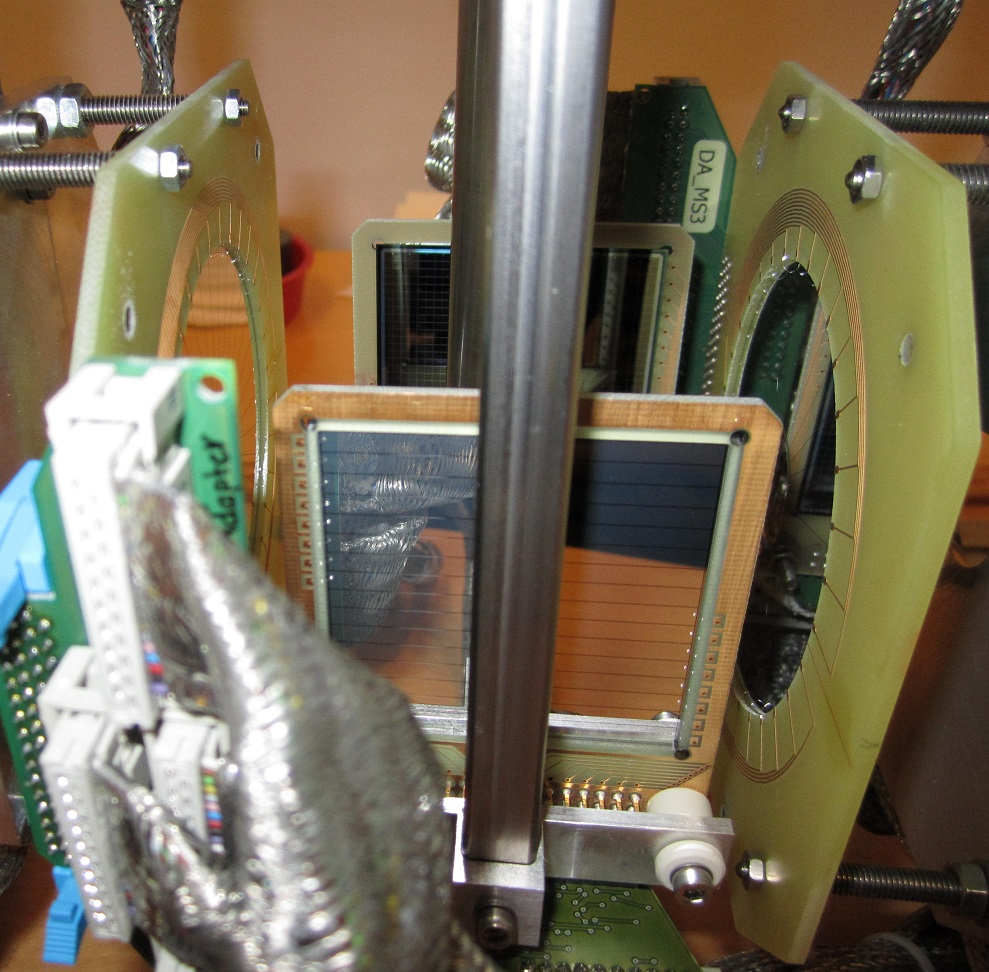
\includegraphics[width=0.4\columnwidth]{realpicture}}
  \caption{}
  \label{fig:detektordistro}
  \vspace{-1cm}
\end{figure}


Detektorerne er forbundet til en forforstærker, der er placeret nær detektoren for at undgå
støj. Signalet fra disse er ført videre til en analog-til-digital konverter (ADK) som til sidst er
ført til computeren. Endvidere er signalerne ført ind i et logisk kredsløb. Udgangssignalet fra
denne bruges som triggersignal til ADK'erne, som så åbnes i \SI{1.4}{\micro\s}. Detektionerne inden
for denne tid kaldes samlet en hændelse og når tiden er ovre, foretages konverteringen og mens denne
foregår, kan der ikke foretages nye detektioner. Det logiske kredsløb har to indstillinger: \lAND og
\lOR. Er den indstillet på \lAND, skal der være signal i mindst to forskellige detektorer før der
kommer et udgangssignal, hvor der ved \lOR kun skal være signal i en enkelt. Dette gør det muligt at
grovsortere således, at de fleste Rutherfordspredte protoner ikke medtages i det endelige datasæt.
